\chapter{Grundlagen neuronaler Netze}
\label{kapitel_neuralnetworks}

In diesem Kapitel werden Künstliche Neuronale Netze\cite{dayhoff1990neural}, kurz KNN, als Forschungsgegenstand der Informatik eingeführt und deren mathematische Grundlagen präzisiert. 
Sie stellen informationsverarbeitende Systeme nach dem Vorbild von tierischen beziehungsweise menschlichen Gehirnen dar und bestehen aus Neuronen in gewissen Zuständen und Schichten, die über gewichtete Verbindungen miteinander gekoppelt sind. Jene Gewichte sind als freie Parameter des neuronalen Netzes zu verstehen und können während des Trainingsprozesses so angepasst werden, um eine entsprechende Aufgabe zu lösen.  
Gelingt dies, so können neuronale Netze genutzt werden, um bestimmte Muster in Daten, typischerweise in Bildern, Audio oder Stromdaten, zu erkennen\cite{pandya1995pattern, pao1989adaptive, urbaniak2021quality}.
Sie eignen sich daher für viele typische Aufgaben des maschinellen Lernens, beispielsweise für die Klassifikation digitalisierter Objekte.

Im ersten Abschnitt wird das Perzeptron\cite{rosenblatt1958perceptron} als Grundeinheit eines neuronalen Netzes eingeführt. 
Im folgenden Abschnitt wird das Konzept der Multi-Layer-Perzeptronen\cite{werbos1988generalization} durch die Kopplung mehrerer Perzeptronen mit bestimmten Übertragungs- und Aktivierungsfunktion in einem Netz erläutert. Diese Repräsentierung eines KNN wird im weiteren Verlauf dieser Arbeit genutzt. Weiter wird das Training neuronaler Netze hinsichtlich der Klassifikationsaufgabe im Abschnitt \ref{abs:task_training} erläutert und schließlich eine kurze Zusammenfassung \ref{abs:NN_conc} gegeben.

\section{Das Perzeptron}
\label{perzeptron_abs}
Zunächst wird das \textit{Perzeptron} ähnlich wie in Minsky \cite{minsky2017perceptrons} als fundamentaler Baustein eines neuronalen Netzes eingeführt. Das Perzeptron wird oft als Basis moderner KNN angeführt und kann mithilfe des Perzeptron-Lernalgorithmus\cite{rosenblatt1958perceptron} trainiert werden, um das Problem der linearen Trennbarkeit \ref{prob:lin_trenn}von Punktmengen zu lösen.
\begin{defi}[Perzeptron]
    \label{def_neuron}
    Für eine gegebene Funktion $\psi: \RR \rightarrow \RR$, einen Vektor $w \in \Rnv$ und ein Skalar $\theta \in \RR$ wird die Funktion 
    \[ \
    \Psi: \RR^n \rightarrow \RR, \; \; \; x \mapsto \psi(w^T x +\theta)=:y,
    \]
    \textit{Perzeptron} genannt. Mit $x \in \Rnv$ wird die vektorwertige Eingabe und mit $y \in \RR$ die skalare Ausgabe des Perzeptrons bezeichnet. Dabei ist mit $w^Tx=\sum_{i=1}^n w_i x_i$ das Standardskalarprodukt im euklidischen Vektorraum $\Rnv$ gemeint. Die Komponenten von $w$ werden Gewichte und der Skalar $\theta$ Schwellwert oder auch Bias genannt.
\end{defi}
Die Funktionsweise eines Perzeptrons ist in Abbildung \ref{funktionsweise_neuron} dargestellt.
\begin{figure}[h]
    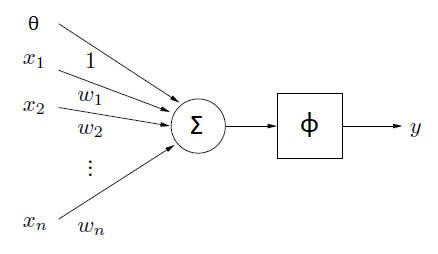
\includegraphics[width=0.8\textwidth]{pics/chapter_neuralnetworks/perzeptron.png}
    \centering
    \caption{Arbeitsweise eines Perzeptrons mit entsprechender Notation aus Definition \ref{def_neuron}.}
    \label{funktionsweise_neuron}
\end{figure}
Bei der Wahl der Funktion $\psi$ gibt es mehrere Möglichkeiten. Wird wie in Minsky\cite{minsky2017perceptrons} die Heavyside-Funktion
\begin{equation*}
    \psi: \RR \rightarrow \RR, \; \; \;
    \psi(x)=\begin{cases}
       1 , \; x \geq 0 \\
       0 , \; \text{sonst}
    \end{cases}
\end{equation*} 
genutzt, kann das Perzeptron als binärer Klassifikator wie in \ref{abs_linear_trenn} interpretiert werden. Dabei dient $w^Tx+\theta=0$ als trennende Hyperebene. Ist $w^Tx+\theta<0$, so ist $\psi(x)=0$ und $x$ wird der Klasse $K_{-1}$ zugeordnet. Gilt jedoch $w^Tx+\theta \geq 0$ und damit $\psi(x)=1$, so ist der Vektor $x$ der Klasse $K_1$ zugehörig. 

Für ein Klassifikationsproblem, bei dem die Klassen nicht linear trennbar sind, scheitern diese einfachen Perzeptronen. Hier wird oft das zweidimensionale XOR-Problem angeführt, bei denen die Punktmengen $P_{-1}=\{(0,0),(1,1)\}$ und $P_{1}=\{(1,0),(0,1)\}$ getrennt werden sollen. Um solche Aufgaben zu lösen, ist es notwendig, mehrere Perzeptronen geschickt zu verknüpfen, um komplexe Entscheidungsgrenzen zu erhalten.

\section{Multi-Layer-Perzeptron}
\label{MLP_abs}
In dieser Arbeit wird ein Künstliches Neuronales Netz als eine Menge von Perzeptronen, die in gewissen Schichten partitioniert und miteinander verbunden sind, notiert. Diese sogenannten \textit{Multi-Layer-Perzeptronen}, kurz MLP,  gelten als erste tiefe neuronale Netze und sind seit den späten 1980er-Jahren Gegenstand der Forschung\cite{bourlard1990links,bounds1988multilayer,MLPbook}. Zunächst sind einige Definition notwendig, um eine lesbare Notation des MLPs zu geben.

\begin{defi}[Übertragungsfunktion]
    \label{def_net}
    Für eine gegebene Matrix $W \in \RR^{n \times m}$ und einen Vektor $b \in \RR^m$ ist 
    \[ 
    \Psi^{W,b}: \RR^n \rightarrow \RR^m, \; \; \; x \mapsto W^T x +b
    \]
    als Übertragungsfunktion definiert. Der Vektor $y=\Psi^{W,b}(x) \in \RR^m $ wird als Netzeingabe bezeichnet.
\end{defi}
Hierbei ist $W$ eine Gewichtsmatrix und $b$ ein Biasvektor, welche als freie Parameter fungieren und die Netzeingabe eines Eingabevektors $x \in \RR^n$ auf lineare Art und Weise beeinflussen. Um auch nichtlineare Zusammenhänge darzustellen, werden Aktivierungsfunktionen benutzt.

\begin{defi}[Aktivierungsfunktion]
    \label{def_act_f}
    Eine stetige, monoton steigende und nicht notwendigerweise lineare Funktion $\psi: \RR \rightarrow \RR$ wird als Aktivierungsfunktion bezeichnet.
\end{defi}
Es sei erwähnt, dass auch nicht monotone Aktivierungsfunktionen genutzt werden können, beispielsweise radiale Basisfunktionen\cite{radialbasis}, welche jedoch in dieser Arbeit nicht weiter von Interesse sind.
Typische Aktivierungsfunktionen, weclhe heutzutage verwendet werden, sind die:
\begin{align*}
    \text{Identität}: \; \;\psi(x)&=x, \\
    \text{Logistische Funktion}: \; \;\psi(x)&=\frac{1}{1+\mathrm{e}^{-x}}, \\
    \text{Tangens Hyperbolicus}: \; \;\psi(x)&=\tanh(x), \\
    \text{ReLU (rectified linear unit)}: \; \;\psi(x)&=\max\{0,x\}.
\end{align*}

\begin{bem}
    Ist $\psi$ eine Aktivierungsfunktion, so wird für $x \in \RR^n$ mit 
    \[\psi(x):=\left(\psi(x_1), \ldots, \psi(x_n)\right)^T \in \RR^n
    \]
    der Vektor bezeichnet, welcher sich durch die elementweise Auswertung der Aktivierungsfunktion $\psi$ an den Stellen $x_1, \ldots, x_n$ ergibt. 
\end{bem}

Bei Klassifikationsproblemen wird oft die \textit{Softmax}-Funktion\cite{denker1990transforming} genutzt, welche die gesamte Eingabe berücksichtigt. Im Abschnitt \ref{task_training} wird erläutert, warum sich in diesem Fall die Softmax-Funktion eignet.

\begin{defi}[Softmax-Funktion]
    Für $x \in \RR^n$ wird die Funktion $\psi: \RR^n \rightarrow (0,1]^n$ mit 
    \[
        \psi(x):=\left(\frac{\mathrm{e}^{x_1}}{\sum_{i=1}^n \mathrm{e}^{x_i}}, \ldots,\frac{\mathrm{e}^{x_n}}{\sum_{i=1}^n \mathrm{e}^{x_i}} \right)^T
    \]
    als Softmax-Funktion definiert. Die Einträge des Vektors $\psi(x)$ summieren sich zu Eins.  
\end{defi}

Für den späteren Trainingsprozess ist es nützlich, die Ableitung der verwendeten Aktivierungsfunktion, sofern sie existiert, zur Verfügung zu haben. Zudem ist es möglich, für bestimmte Aktivierungsfunktionen die Ableitung nur mithilfe der verwendeten Funktion zu berechnen.

\begin{lem}
    \begin{itemize}
        \item[(i)] Für die ReLU $\psi(x)=\max\{0,x\}$ gilt
         \[\psi'(x)=\begin{cases}
            0 &, x <0 \\
            1 &, x >0
        \end{cases}. 
        \]
        An der Stelle 0 ist die Ableitung nicht definiert und wird oft mit $\psi'(0)=\frac{1}{2}$ festgelegt.
        \item[(ii)] Für die logistische Funktion $\psi(x)=\frac{1}{1+\mathrm{e}^{-x}}$ gilt
        \[ 
            \psi'(x)=\psi(x)(1-\psi(x)) 
        \]
        für alle $x \in \RR$.
        \item[(iii)] Für den Tangens Hyperbolicus $\psi(x)=\tanh(x)$ gilt
        \[ 
            \psi'(x)=1-\psi^2(x) 
        \]
        für alle $x \in \RR$.
    \end{itemize}
\end{lem}
\begin{proof}
    Einfaches Differenzieren liefert für $(i)$ und $(ii)$ die Resultate. Bei $(iii)$ wird die Darstellung $\tanh(x)=\frac{2}{\mathrm{e}^{2x}+1}$ genutzt und das Differenzieren mittels Quotientenregel liefert die Aussage.
\end{proof}


Ähnlich der Definition des Perzeptrons \ref{def_neuron} wird nun eine Schicht als Verknüpfung von Übertragungsfunktion und Aktivierungsfunktion definiert.

\begin{defi}[Neuronenschicht]
    \label{def:NNlayer}
    Ist $\Psi^{W,b}$ eine Übertragungsfunktion mit den Parametern $W \in \RR^{n \times m}, b \in \RR^m$ und $\psi$ eine Aktivierungsfunktion, so wird das Paar $(\Psi^{W,b}, \psi)$ als Schicht $\mathcal{S}$ bezeichnet. Für eine Eingabe $x \in \RR^n$ ist die Ausgabe $y \in \RR^m$ der Schicht $\mathcal{S}$ durch
    \[y=\psi \circ \Psi^{W,b}(x)= \psi\left(\Psi^{W,b}(x)\right)
        \] 
        gegeben. Die Komponenten $y_i$ werden für $1 \leq i \leq m$ Neuronen der Schicht $\mathcal{S}$ genannt und gleichen jeweils der Ausgabe eines einfachen Perzeptrons wie in Definition \ref{def_neuron}. Eine Schicht besteht aus $m$ Perzeptronen $\tilde{\Psi}_i$ mit $y_i=\tilde{\Psi}(x_i)=\psi(W_{i,:}^T x+b_i)$ für $1 \leq i \leq m$.
\end{defi}
Im Hinblick auf MLPs werden nun mehrere Schichten so verbunden, dass die Ausgabe einer Schicht $\mathcal{S}_k$ als Eingabe einer darüberliegenden Schicht $\mathcal{S}_{k+1}$ für ein $k \in \mathbb{N}$ dient. Die Anzahl der Neuronen kann dabei von Schicht zu Schicht variieren. Dementsprechend werden die Dimensionen der beteiligten Gewichtsmatrizen $W^{(k)}$ und Biasvektoren $b^{(k)}$ passend gewählt. 
Um die Notation übersichtlich zu halten, bezeichne $\Psi^{W^{(k)},b^{(k)},\psi_{k}}$ die Schicht $\mathcal{S}_k$ mit $\Psi^{W^{(k)},b^{(k)},\psi_{k}}(x):= \psi_{k} \left(\Psi^{W^{(k)},b^{(k)}}(x)\right)$.

\begin{defi}[Multi-Layer-Perzeptron, vgl. gruening]
    \label{def:MLP}
    Für eine gegebene Anzahl $l \in \mathbb{N}, \; l>1$ von Schichten $\Psi^{W^{(1)},b^{(1)},\psi_{1}}, \ldots, \Psi^{W^{(l)},b^{(l)},\psi_{l}}$ bezeichne $s_l \in \mathbb{N}$ die Anzahl der Neuronen in Schicht $l$. Für eine Eingabe $x \in \RR^{s_0}$ lässt sich die Ausgabe $y \in \RR^{s_l}$ eines Multi-Layer-Perzeptron  $\Lambda_l: \RR^{s_0} \rightarrow \RR^{s_l}, \; x \mapsto y$ mit $l$ Schichten durch
    \[
        y=\Psi^{W^{(l)},b^{(l)},\psi_{l}} \circ \ldots \circ \Psi^{W^{(1)},b^{(1)},\psi_{1}}(x)
    \]
    berechnen. Dabei gelten für die Gewichtsmatrizen die Dimensionsbedingungen
    \[{}_1W^{(1)}=s_0, \; \; {}_2W^{(l)}=s_l, \; \; \forall i \in [l-1]: \; {}_2W^{(i)}={}_1W^{(i+1)}.
        \] 
    Die Eingabeschicht $\mathcal{S}_0$ besitzt keine Parameter $W$ und $b$ und besteht nur aus dem Eingabevektor $x \in \RR^{s_0}$. Die letzte Schicht $\Psi^{W^{(l)},b^{(l)},\psi_{l}}$ wird als Ausgabeschicht bezeichnet. Weiter werden die Schichten $\mathcal{S}_1, \ldots, \mathcal{S}_{l-1}$ als verdeckte Schichten definiert. Das MLP wird auch Feed-Forward-Netz (FFN)  genannt und die Funktionsauswertung $\Lambda_l(x)$ für eine Eingabe $x$ wird mit Vorwärtsrechnung, engl. \textit{forward propagation}, bezeichnet.
\end{defi}

\begin{algorithm}
    \caption{Vorwärtsrechnung}\label{alg:ff}
    \begin{algorithmic}
    \Require $ \text{MLP} \; \Lambda_l, \text{Eingabe} \; x_0 \in \RR^n$
    \Ensure $y = \Lambda_l(x) \in \RR^m$
    \State $x=x_0$
    \For{$i=1, \ldots l}$
    \State $u=W^{(i) \,T}x+b^{(i)}$
    \State $x=\psi_i(u)$
    \EndFor
    \State $y=x$
    \end{algorithmic}
\end{algorithm}
    


Das MLP-Modell wird im weiteren Verlauf dieser Arbeit repräsentativ als Künstliches Neuronales Netz bezeichnet. Die Begriffe MLP und FFN sind austauschbar. Die Funktionsauswertung eines FNN wird im Algorithmus Vorwärtsrechnung \ref{alg:ff} festgehalten. Das zuvor angesprochene XOR-Problem kann nun beispielsweise mithilfe eines KNN bestehend aus zwei Schichten gelöst werden\cite{Goodfellow-et-al-2016}.
Es lassen sich zwischen Modell- und Hyperparameter von KNN unterscheiden.

\begin{defi}[Hyper- und Modellparameter]
    Sei für $l \in \mathbb{N}$ ein KNN $\Lambda_l$ gegeben. Dann werden die Eingabe- und Ausgabedimension $s_0, s_l$, die Anzahl $l$ der (verdeckten) Schichten sowie die verwendeten Aktivierungsfunktion $\psi_l$ Hyperparameter des neuronalen Netzes genannt.
    Die Gewichtsmatrizen und Biasvektoren mit den entsprechend passenden Abmessungen stellen die Modellparameter $\mathcal{W}:=\{(W^{(i)},b^{(i)}): \; i=1, \ldots, l\}$ des neuronales Netzes dar. 
\end{defi}
Die Hyperparameter werden oft anwendungsspezifisch für das jeweilige Problem gewählt, während die Modellparameter dynamisch in einem Trainingsprozes angepasst werden, sodass die gegebene Aufgabe zufriedenstellend gelöst wird. Wie dies geschieht, wird im folgenden Abschnitt \ref{task_training} erläutert.

\section{Training neuronaler Netze}
\label{abs:task_training}
Künstliche Neuronale Netze gehören zu den typischen Vertretern von maschinellen Lernalgorithmen, welche hinsichtlich einer bestimmten Aufgabe, engl. \textit{task T}, und einem Leistungsmaß, engl. \textit{perfomance P} an der Erfahrung, engl. \textit{experience E} lernen\cite{Goodfellow-et-al-2016}. Dabei ist mit Lernen gemeint, dass das Computerprogramm bezüglich der Aufgabe $T$ sein Leistungsmaß $P$ mit wachsener Erfahrung $E$ schrittweise steigert. Wie in Kapitel \ref{fund} erläutert, gibt es viele verschiedene Aufgaben, wie die Regression, Klassifikation oder Clusterung bestimmter Objekte. 

In den folgenden Abschnitten wird das Klassifikationsproblem als \textit{task T} im Mittelpunkt stehen. Weiter werden KNNs als Modellschätzer aus der Wahrscheinlichkeitstheorie interpretiert und fundamentale Aussagen wie das \textit{Universal-Approximation-Theroem}\cite{HORNIK1989359} gegeben. Schließlich wird bezüglich der Klassifikationsaufgabe das Training neuronaler Netze erläutert.


\subsection{Neuronale Netze als universelle Schätzer}
\label{NN_estimators_abs}
Beim Klassifikationsproblem müssen bestimmte bedingte Wahrscheinlichkeiten, die in diesem Abschnitt erklärt werden, ermittelt werden. Oft wird dazu die Ausgabeschicht eines KNN als Wahrscheinlichkeit interpretiert und daher KNN als Schätzer der bedingten Wahrscheinlichkeiten eingesetzt. Zunächst werden Klassifikationsfunktion und -problem definiert.
\begin{defi}
    \label{def_classfun}
    Seien die Mengen $D \subset \RR^n$ und $\mathcal{C}=\{c_1, \ldots, c_m\}$ gegeben. Eine Funktion $f: D \rightarrow \mathcal{C}$, welche ein Element aus $D$ einer Klasse $c_i \in \mathcal{C}$ zuordnet, wird Klassifikationsfunktion genannt. Hier gibt es $m \in \mathbb{N}$ verschiedene Klassenlabels.
\end{defi}

Das Ziel beim Klassifikationsproblem ist die Approximation einer nicht bekannten Klassifikationsfunktion $f:D \rightarrow \mathcal{C}$ durch ein Modell $\tilde{f}: D \rightarrow \mathcal{C}$. 
In dieser Arbeit werden dafür KNNs genutzt, welche als probabilistische Modelle auf folgende Weise genutzt werden. Auf der Ergebnismenge $\Omega= D \times \mathcal{C}$ sei die nicht bekannte gemeinsame (Wahrscheinlichkeits-) Verteilung $p_{Daten}(x,c)$, genannt Datenverteilung, gegeben. Ein Modell soll nun konstruiert werden, welches die a posterior-Verteilung $p_{Daten}(\cdot \; | \; x)$ der Klassen schätzt. 

In dieser Arbeit werden KNN so benutzt, dass die Klassenzugehörigkeit direkt anhand der Eingabe $x \in D$ geschätzt wird. Die Funktion $P_{Daten}: D \rightarrow [0,1]^m$ mit
\begin{equation}
    \label{eq:Pdaten}
    P_{Daten}(x):=\left(p_{Daten}(c_1 \; | \; x), \ldots, p_{Daten}(c_m \; | \; x)\right)^T \in \RR^m
\end{equation} soll für alle $x \in D$ approximiert werden. Dazu wird die Funktion $P_{Modell}: D \rightarrow [0,1]^m$ mit 
\begin{equation}
    \label{eq:Pmodell}
    P_{Modell}(x;\mathcal{W}):=\left(p_{Modell}(c_1 \; | \; x; \mathcal{W}), \ldots, p_{Modell}(c_m \; | \; x; \mathcal{W})\right)^T \in \RR^m
\end{equation}
 für alle $x \in D$  genutzt, welche von den Modellparametern $\mathcal{W}$ abhängig ist. Die Klassifikationsfunktion des Modells ergibt sich als
\begin{equation}
    \label{eq:f_modell}
    f_{Modell}(x):= \underset{c \in \mathcal{C}}{\mathrm{argmax}} \; p_{Modell}(c \; | \; x).
\end{equation}

Es stellt sich die Frage, inwiefern das MLP als Modell genutzt werden kann, um beliebige Datenverteilungen $P_{Daten}$ zu approximieren. Folgende Resultate liefern die Antwort.

\begin{satz}[Universal-Approximation-Theroem\cite{gruen}]
    \label{UAT}
    Sei $\psi_1$ eine nichtkonstante, beschränkkte Aktivierungsfunktion und $id: \RR \rightarrow \RR$ die Identität sowie $D \subset \RR^n$ kompakt. Dann existieren für alle $\varepsilon >0$ und stetigen Funktionen $f: D \rightarrow \RR$ Parameter $N \in \mathbb{N}, W^{(1)} \in \RR^{n \times N}, b^{(1)} \in \RR^N$ sowie $W^{(2)} \in \RR^{N \times 1}$, sodass
    \begin{equation}
        \label{UAP_eq}
        \left|f(x)-\Psi^{W^{(2)},0,id} \circ \Psi^{W^{(1)},b^{(1)},\psi_1}(x)\right| < \varepsilon, \; \; \forall x \in D
    \end{equation}
    gilt.
\end{satz}

\begin{proof}
    Ein Beweis kann in Hornik\cite{hornik1991approximation} nachgelesen werden.
\end{proof}

Das Universal-Approximation-Theroem kann ebenfalls auf unbeschränkte und nichtkonstante Funktion $f:D \rightarrow \RR^m$ erweitert werden. Heutzutage wird oft die ReLU-Funktion als Aktivierungsfunktion verwendet\cite{schmidt2020nonparametric,li2017convergence}.

\begin{kor}
    Mit den gleichen Vorraussetzungen wie in Satz \ref{UAT} gilt die Abschätzung \ref{UAP_eq} für $\psi_1(x)=\max\{0,x\}$.
\end{kor}

\begin{proof}
    Siehe Sonoda et. al.\cite{sonoda2017neural}.
\end{proof}

Hinsichtlich der Approximation von beliebigen Funktionen $P_{Daten}$ mithilfe eines neuronalen Netzes mit der Softmax-Funktion als Aktivierungsfunktion liefert Strauß\cite{strauss} folgendes Resultat.

\begin{kor}
    \label{kor_softmax}
    Ein MLP mit zwei Schichten, wobei $\psi_2$ die Softmax-Funktion ist, kann genutzt werden, um stetige Funktionen $f:K \rightarrow [0,1]^m$, welche von einem Kompaktum $K \subset \RR^n$ in eine (Wahrscheinlichkeits)-Verteilung über die Klassen $\mathcal{C}$ abbilden, beliebig genau zu approximieren.
\end{kor}

\begin{proof}
    Siehe \cite{strauss}.
\end{proof}

Die Aussage kann auf das MLP mit beliebig vielen Schichten erweitert werden.
In dieser Arbeit umfasst die Menge $D$ aus Definition \ref{def_classfun} digitalisierte Objekte als Vektoren $x \in \RR^n$ und ist endlich und damit kompakt. Daher kann wegen Korollar \ref{kor_softmax} das MLP als Modell genutzt werden, um stetige Funktionen $P_{Daten}$ sinnvoll zu approximieren.

\subsection{Optimale Parameterwahl bei neuronalen Netzen}

Wird ein künstliches neuronales Netz als probabilistisches Modell genutzt und sind die Hyperparameter festgelegt, müssen die Modellparameter $\mathcal{W}$ gewählt werden. Um die Approximationsgüte, also die \textit{perfomance P}, bezüglich des Klassifikationsproblems messbar zu machen, werden Fehlerfunktionen eingeführt. 
Mit Trainingsdaten als \textit{experience E} und dem Gradientenverfahren\cite{nocedal1999numerical} sollen optimale Parameter $\mathcal{W}$ gefunden werden, sodass die gewählte Fehlerfunktion minimiert wird. Im folgenden steht ein MLP $\Lambda(\, \cdot \, ; \mathcal{W}): D \rightarrow [0,1]^m$  mit der Softmax-Funktion als Aktivierungsfunktion im Mittlepunkt, welches als parametrisiertes Modell $f_{Modell}$ wie in \ref{eq:f_modell} genutzt wird.
Die Trainingsdaten werden in Trainingsmengen und Testmengen aufgeteilt.

\begin{defi}[Trainingsmenge, Testmenge]
    Sei $p_{daten}$ eine Datenverteilung auf der Ergebnismenge $\Omega=D \times \mathcal{C}$. Dann heißen für $n_{train}, n_{test} \in \mathbb{N}$ die Mengen
    \begin{align*}
        \mathcal{T} &:= \left\{ (x^{(i)},c^{(i)}) \; | \; i \in [n_{train}] \right\} \subset \Omega \\
        \mathcal{T}' &:= \left\{ (x^{(i)},c^{(i)}) \; | \; i \in [n_{test}] \right\} \subset \Omega
    \end{align*}
    Traingsmenge $\mathcal{T}$ und Testmenge $\mathcal{T}'$, jeweils bestehend aus Datenpaaren, welche unabhängig durch $p_{Daten}$ generiert wurde. Oft werden die Mengen disjunkt gewählt. Die Menge $\mathcal{T}$ wird zum Trainieren und die Menge $\mathcal{T}'$ zur Validierung des Modells $P_{Modell}$ bezüglich $P_{Daten}$ wie in \ref{eq:Pdaten} genutzt.
\end{defi}

Die Approximationsgüte des Modells $f_{Modell}$ wird als Likelihood gegeben einer Trainingsmenge $\mathcal{T}$ gemessen und lässt sich als 

\begin{equation}
    \label{eq:likelihood}
    L(\mathcal{T},\mathcal{W}):=\prod_{(x,c) \in \mathcal{T}} p_{Modell}(c \; | \; x; \mathcal{W})
\end{equation}
wie in Bishop\cite{bishop2006pattern} berechnen.
Für eine Trainingsmenge $\mathcal{T}$ soll das Produkt über alle Wahrscheinlichkeiten der korrekten Klassenzugehörigkeiten $c$ gegeben der Eingaben $x$ maximiert werden. Dieser Ansatz wird \textit{Maximum Likelihood-Methode}\cite{ruschendorf2014mathematische} genannt und eine Parameterwahl ist durch eine Lösung des Optimierungsproblems 
\begin{equation}
    \label{eq:opt_likelihood}
     \prod_{(x,c) \in \mathcal{T}} p_{Modell}(c \; | \; x; \mathcal{W}) \rightarrow \max
\end{equation}
gegeben. Dabei sei bemerkt, dass die Optimierung unabhängig von den Hyperparametern vorgenommen wird.

Für ein Trainingspaar $(x,c) \in \mathcal{T}$ bezeichne $t(x,c) \in \RR^m$ den Zielvektor der Klasse $c$ mit sogenannter (1 aus m)-Kodierung. Die Komponenten des Zielvektors sind
\begin{equation*}
    t_k(x,c):= \begin{cases}
        1 &, \text{wenn} \; k=c \\
        0 &, \text{sonst}
    \end{cases}, \; \; \forall k \in [m].
\end{equation*} 
Mit dieser Bezeichnung lässt sich das Optimierungsproblem \ref{eq:opt_likelihood} als Minimierungproblem mithilfe der \textit{negative log likelihood} schreiben.
\begin{defi}[negative log likelihood]
    Seien die Mengen $D$ und  $\mathcal{C}=\{c_1, \ldots, c_m\}$ mit einer dazugehörigen Trainingsmenge $\mathcal{T}$ sowie entsprechende Zielvektoren gegeben. Weiter seien die a posterior Wahrscheinlichkeiten $p_{Modell}(c \; | \; x; \mathcal{W})$ wie in Gleichung \ref{eq:Pmodell} gegeben. Die negative log likelihood ist als Funktion 
    \begin{equation}
        \label{eq:NLL}
        L_{NNL}(\mathcal{T},\mathcal{W}):= -\sum_{(x,c) \in \mathcal{T}}  \sum_{i=1}^m t_i(x,c) \log \left(p_{Modell}(c_i \; | \; x; \mathcal{W}) \right) 
    \end{equation}
    definiert.
\end{defi}

Das Minimieren der negative log likelihood ist äquivalent zur Maximierung der Likelihood aus \ref{eq:likelihood}, denn es gilt 
\begin{equation*}
    \log \left(\prod_{(x,c) \in \mathcal{T}} p_{Modell}(c \; | \; x; \mathcal{W})\right)= \sum_{(x,c) \in \mathcal{T}} \log \left(p_{Modell}(c \; | \; x; \mathcal{W}) \right)
\end{equation*}
und der natürliche Logarithmus ist monoton steigend. Wird zusätzlich angenommen, dass die a posterior Verteilung  $p_{Daten}(c \; | \; x)$ einer Normalverteilung mit konstanter Varianz entspricht, so ist das Maximieren von \ref{eq:likelihood} äquivalent zur Minimierung der mittleren quadratischen Abweichung
\begin{equation*}
    \label{eq:MSE}
    L_{MSE}(\mathcal{T},\mathcal{W}):=\frac{1}{2} \sum_{(x,c) \in \mathcal{T}} ||\hat{c}-t(x,c)||_2^2,
\end{equation*}
wobei $\hat{c}=f_{Modell}(x)$ und $t(x,c)$ der Zielvektor des Datenpaars $(x,c)$ ist, siehe Goodfellow\cite{Goodfellow-et-al-2016}. 
Das Problem \ref{eq:opt_likelihood} wird nun allgmemein mit Fehlerfunktionen definiert.
 \begin{defi}[Fehlerfunktion]
    Seien $\mathcal{T}$ eine Trainingsmenge und $\mathcal{W}$ Modellparameter eines KNN. Mithilfe des Gradientenverfahrens soll das Problem
    \begin{equation}
        \label{eq:error_fun_opt}
        \mathcal{E}(\mathcal{T},\mathcal{W}) \rightarrow \min
    \end{equation}
    gelöst werden. Dabei wird $\mathcal{E}$ Fehlerfunktion gennant.
 \end{defi}
In dieser Arbeit wird $\mathcal{E}$ immer als stückweise stetig differenzierbare Funktion gewählt, damit das Gradientenverfahren angewendet werden kann. Sowohl die negative log likelihood $L_{NNL}$ als auch die mittlere quadratische Abweichung $L_{MSE}$ sind als Fehlerfunktion geeignet.
Die Optimierung der Parameter geschieht iterativ und besteht jeweils aus zwei Schritten. Zuerst wird eine Abstiegsrichtung 
\begin{equation}
    \label{eq:gradE}
    \Delta_n :=\nabla_{\mathcal{W}} \mathcal{E}(\mathcal{T},\mathcal{W})
\end{equation} 
berechnet und dann die Parameter 
\begin{equation}
    \label{eq:step}
    \mathcal{W}_{n+1}:=\mathcal{W}_n- \lambda \Delta_n
\end{equation}
aktualisiert. Es werden also Gradienten der Fehlerfunktion bezüglich der Gewichtsmatrizen und Biasvektoren ermittelt und anschließend werden jene Parameter mit einer wählbaren Lernrate $\lambda \in \RR$ angepasst. In \ref{eq:gradE} wird der Gradient über alle Trainingspaare berechnet. Diese Variante nennt sich \textit{Offline-Version} des Gradientenverfahrens und ist besonders für große Trainingsmengen ineffizient. Die \textit{Online-Version} berechnet den Gradienten lediglich für ein Trainingspaar und passt die Parameter direkt an. In dieser Arbeit wird ein Kompromiss aus beiden Verfahren verwendet und zwar das \textit{Mini-Batch-Verfahren}, siehe Algorithmus \ref{alg:minibatch}, bei dem die Gradienten über kleine Teilmengen $\mathbb{T} \subset \mathcal{T}$ der Trainingsmenge berechnet werden.

\begin{algorithm}
    \caption{Mini-Batch-Verfahren, vgl. \cite{gruening}}\label{alg:minibatch}
    \begin{algorithmic}
    \Require $ \text{Trainingsmenge} \; \mathcal{T}, \text{Modellparameter} \; \mathcal{W}_0, \text{Fehlerfunktion} \; \mathcal{E}, \text{Batch-Größe} \; n$
    \Ensure $\text{optimierte Modellparamter} \; \mathcal{W}$
    \State $\mathcal{W}=\mathcal{W}_0$
    \State $\mathbb{T}=\mathcal{T}$
    \State Setze Lernrate $\lambda$ \Comment{Wahlmöglichkeiten, siehe Text}     
    \While{Abbruchbedingung nicht erfüllt} \Comment{Abbruchbedingung, siehe Text}
    \If{$|\mathbb{T}| < n$}
        \State $\mathbb{T}=\mathcal{T}$
    \EndIf
    \State $\mathbb{T}_n=$ zufällig gewählte $n$ Datenpaare von $\mathbb{T}$ 
    \State $\mathcal{W}=\mathcal{W}-\lambda \nabla_{\mathcal{W}} \mathcal{E}(\mathbb{T}_n,\mathcal{W})$
    \State $\mathbb{T}= \mathbb{T} \setminus \mathbb{T}_n$
    \EndWhile
    \end{algorithmic}
\end{algorithm}

Als Abbruchbedingung im Mini-Batch-Verfahren kann eine fest gewählte Anzahl von Updateoperationen der Parameter gewählt werden. Andere Abbruchbedingungen können mit der Norm der Abstiegsrichtungen\cite{bishop2006pattern} oder abhängig vom Traingsfehler formuliert werden. Bei der Wahl der Lernrate werden heutzutage werden oft adaptive Verfahren genutzt, welche vorangegangene Gradienten berücksichtigen und die Lernrate so anpassen. Bekannte Verfahren sind \textit{Nesterov accelerated
gradient}\cite{sutskever2013importance}, \textit{AdaGrad}\cite{duchi2011adaptive}, \textit{RMSProp}\cite{tieleman2012lecture} sowie \textit{Adam}\cite{Kingma2015AdamAM}. So sollen Probleme wie des \textit{vanishing gradients} oder des \textit{exploding gradients} vermieden werden\cite{hanin2018neural}.
Für eine tiefere Analyse des Gradientenverfahrens und dessen Varianten sei auf die jeweilgen Arbeiten beziehungsweise Ruder\cite{ruder2016overview,} verwiesen. Darüber hinaus gibt es andere Techniken wie die Regularisierung, um Probleme wie Überanpassung, engl.\textit{overfitting}, zu entgegnen.
Für die Problemstellung in dieser Arbeit genügt es, das Mini-Batch-Verfahren mit konstanter Lernrate zu nutzen. 

Die Abstiegsrichtungen werden werden mithilfe der mehrdimensionalen Kettenregel in einer Backpropagationsphase, etabliert von Rumelhart et. al. \cite{MLPbook}, berechnet.
\begin{satz}[Mehrdimensionale Kettenregel]
    \label{chainrule}
    Ist $f=f(x_1(y_1, \ldots, y_m), \ldots, x_n(y_1, \ldots, y_m))$ und sind alle beteiligten Funktionen stetig differenzierbar, so ergeben sich die partielle Ableitungen mittels Kettenregel zu

    \begin{equation*}
        \frac{\partial f}{\partial y_i}=\sum_{j=1}^n \frac{\partial f}{\partial x_i} \frac{\partial x_j}{\partial y_i} .
    \end{equation*}
\end{satz}

\begin{proof}
    siehe \cite{forster2017analysis}
\end{proof}
Im Bereich des tiefen Lernens zählt die effiziente Berechnung dieser Gradienten zu den schwersten Aufgaben. Eine ausführliche Erklärung der Backpropagationsphase für klassische FFN ist beispielsweise in Rojas\cite{rojas96neural} zu finden. 

\section{Zusammenfassung}
\label{abs:NN_conc}
In diesem Kapitel wurden KNN als Feed-Forward-Netze eingeführt. Es stellt sich heraus, dass diese Netze als probabilistische Modelle genutzt werden können, um Klassifikationsaufgaben hinreichend gut zu lösen. Dabei ist es wichtig die Hyper- und Modellparameter je nach Anwendung und Leistungsmaß optimal zu wählen. Dazu werden Trainingsdaten genutzt, um während eines Lernprozesses eine Fehlerfunktion zu Minimieren. Eine Lösung von \ref{eq:error_fun_opt} kann wegen der Komplexität der Fehlerfuntion $\mathcal{E}$ bzw. der großen Menge von Parametern $\mathcal{W}$ selten direkt angegeben werden\cite{blum1992training}. Daher wird das Mini-Batch-Verfahren als iterativer Ansatz zur numerischen Mnimierung der Fehlerfunktion genutzt. Dabei sind partielle Ableitungen der Fehlerfunktion bezüglich der Parameter nötig, welche in der Backpropagationsphase mithilfe der mehrdimensionalen Kettenregel berechnet werden können. 

Bei der Analyse von Zeitreihen oder Bildern eignen sich abgewandelte Architekturen wie gefaltete neuronale Netze (CNN), engl. \textit{convolutional neural networks}, welche im folgenden Kapitel \ref{kap:CNN} näher erläutert werden. Diese Art neuronaler Netze wird im weiteren Verlauf dieser Arbeit im Fokus stehen.


    





